\documentclass[11pts]{beamer}

\usepackage{graphicx}
\usepackage{subfigure}
\usepackage{enumerate}
\usepackage{enumitem}
\usepackage{setspace}
\usepackage[english]{babel}
\usepackage{setspace,psfrag,cite,amsmath,paralist,amssymb}
\usepackage{amsfonts,beamerbasetheorems,epsfig}
\usepackage{graphicx}
\usepackage[T1]{fontenc}
\usepackage{float}
\usepackage{epstopdf}
\usepackage{ragged2e}
\usepackage{ dsfont }
\usepackage{wrapfig}
\usepackage[utf8]{inputenc}
\usepackage{xcolor} 
\usepackage{mathtools}
\usepackage{breqn}
\usepackage{float}
\usepackage[caption = false]{subfig}
\usepackage[demo]{graphicx}
\usepackage{graphicx}
\usepackage{subcaption}

\usepackage{amsmath,amsthm,amsfonts,amssymb,amscd}
\usepackage{lastpage}
\usepackage{enumerate}
\usepackage{fancyhdr}
\usepackage{mathrsfs}
\usepackage{xcolor}
\usepackage{graphicx}
\usepackage{listings}
\usepackage{hyperref}
\usepackage{optidef}


\usepackage{blindtext}
\usepackage[inline]{enumitem}
\usepackage{xcolor}

\usepackage{pgfplots}
\pgfplotsset{ticks=none,width=7cm,compat=1.8}

\DeclareMathOperator*{\argmin}{arg\,min}

\newenvironment{changemargin}[2]{%
\begin{list}{}{%
\setlength{\topsep}{-5pt}%
\setlength{\leftmargin}{#1}%
\setlength{\rightmargin}{#2}%
\setlength{\listparindent}{\parindent}%
\setlength{\itemindent}{\parindent}%
\setlength{\parsep}{\parskip}%
}%
\item[]}{\end{list}}




%% Beamer Layout %%%%%%%%%%%%%%%%%%%%%%%%%%%%%%%%%%
\usepackage{tikz}

\usetheme{Udel} 	
%\usetheme[]{CambridgeUS}
\usepackage{lmodern} 	
%\usepackage{palatino}
%%%%%%%%%%%%%%%%%%%%%%%%%%%%%%%%%%%%%%%%%%%%%%%%%%

\DeclareMathOperator*{\argmax}{arg\,max}
\DeclareMathOperator*{\argmin}{arg\,min}


%%%%%%%%%%%%%%%%%%%%%%%%%%%%% TITLE %%%%%%%%%%%%%%%%%%%%%%%%%%%%%%%%%%%%%%%
\title{\LARGE{A Graph Signal Processing Approach to Active Learning}}%
\author[Maria Dapena\\ Daniel Lau \\ Gonzalo Arce]{\large{Maria Dapena\\Daniel Lau \\ Gonzalo Arce}}
\date{ University of Delaware,\\ Newark, Delaware}
\pgfdeclareimage[height=0.4cm,width=0.3cm]{coat}{coat.pdf}
 \logo{\pgfuseimage{coat}}
 
\usepackage{enumitem,xcolor}
\definecolor{bar}{rgb}{.03,.4,.7}


\usepackage{blindtext}
\usepackage{tcolorbox}
\usepackage{graphicx}
%%%%%%%%%%%%%%%%%%%%%%%%%%%%%%%% BEGIN DOCUMENT %%%%%%%%%%%%%%%%%%%%%%%%%%
\begin{document}
%\beamertemplatenavigationsymbolsempty
\normalsize

%%%%%%%%%%%%%%%%%%%%%%%%%%%%%%%%%%%%%%%%%%%%%%%%%%%%%
%%%%%%%%%%%%%%%%%%%%%%%%%%%%%%%%%%%%%%%%%%%%%%%%%%%%%
\begin{frame}%[Title]
	\titlepage
\end{frame}
%%%%%%%%%%%%%%%%%%%%%%%%%%%%%%%%%%%%%%%%%%%%%%%%%%%%%
%%%%%%%%%%%%%%%%%%%%%%%%%%%%%%%%%%%%%%%%%%%%%%%%%%%%%

%%%%%%%%%%%%%%%%%%%%%%%%%%%%%%%%%%%%%%%%%%%%%%%%%%%%%
%%%%%%%%%%%%%%%%%%%%%%%%%%%%%%%%%%%%%%%%%%%%%%%%%%%%%
\begin{frame}%[Outline]
\frametitle{Outline}
    \begin{enumerate}[\color{bar}\bfseries 1.]
        
        \item Introduction
        \item Active Learning
        \item Graph And Blue Noise
        \item Problem Formulation
        \item Proposed Method
        \item Signal Reconstructions as a Classifier
        \item Experiments and Results 
        \item Conclusion and Future Work

    \end{enumerate}
\end{frame}
%%%%%%%%%%%%%%%%%%%%%%%%%%%%%%%%%%%%%%%%%%%%%%%%%%%%%
%%%%%%%%%%%%%%%%%%%%%%%%%%%%%%%%%%%%%%%%%%%%%%%%%%%%%


%%%%%%%%%%%%%%%%%%%%%%%%%%%%%%%%%%%%%%%%%%%%%%%%%%%%%
%%%%%%%%%%%%%%%%%%%%%%%%%%%%%%%%%%%%%%%%%%%%%%%%%%%%%
\begin{frame}%[Passive ]
\frametitle{Introduction: Passive Learning}
    \begin{figure}
        \centering
        \includegraphics[scale=0.35]{IM/PASIVELEARNING.pdf}
    \end{figure}
\end{frame}
%%%%%%%%%%%%%%%%%%%%%%%%%%%%%%%%%%%%%%%%%%%%%%%%%%%%%
%%%%%%%%%%%%%%%%%%%%%%%%%%%%%%%%%%%%%%%%%%%%%%%%%%%%%



%%%%%%%%%%%%%%%%%%%%%%%%%%%%%%%%%%%%%%%%%%%%%%%%%%%%%
%%%%%%%%%%%%%%%%%%%%%%%%%%%%%%%%%%%%%%%%%%%%%%%%%%%%%
\begin{frame}%[Active]
\frametitle{Introduction: Active Learning}
\begin{tcolorbox}[width=\textwidth,colback={bar}]    
   \textcolor{white}{Is it possible to train machines with less labeled data?}
   
    \textcolor{white}{Can we use less human resources?}
\end{tcolorbox} 

    \begin{figure}
        \centering
        \includegraphics[scale=0.35]{IM/ACTIVELEARNING.pdf}
    \end{figure}
\end{frame}
%%%%%%%%%%%%%%%%%%%%%%%%%%%%%%%%%%%%%%%%%%%%%%%%%%%%%
%%%%%%%%%%%%%%%%%%%%%%%%%%%%%%%%%%%%%%%%%%%%%%%%%%%%%

%%%%%%%%%%%%%%%%%%%%%%%%%%%%%%%%%%%%%%%%%%%%%%%%%%%%%
%%%%%%%%%%%%%%%%%%%%%%%%%%%%%%%%%%%%%%%%%%%%%%%%%%%%%
%\begin{frame}%[Active Scenarios]
%\frametitle{Active Learning: Scenarios}
%Three main scenarios:
%\begin{enumerate}[\color{bar}\bfseries $\bullet$]
%    \item Membership query synthesis: The model generates a new sample.
%    \item Stream-based selective sampling: sample a instance and the model decides to discard or no
%    \item Pool-based sampling: select  $\mathcal{U}$ samples from the unlabeled pool and the model select the best query
%\end{enumerate}
%\begin{figure}[h]
%        \centering
%        \includegraphics[scale=0.25]{IM/SCE.png}
 %   \end{figure}
    
%\end{frame}
%%%%%%%%%%%%%%%%%%%%%%%%%%%%%%%%%%%%%%%%%%%%%%%%%%%%%
%%%%%%%%%%%%%%%%%%%%%%%%%%%%%%%%%%%%%%%%%%%%%%%%%%%%%



%%%%%%%%%%%%%%%%%%%%%%%%%%%%%%%%%%%%%%%%%%%%%%%%%%%%%
%%%%%%%%%%%%%%%%%%%%%%%%%%%%%%%%%%%%%%%%%%%%%%%%%%%%%
\begin{frame}%[Active Query]
\frametitle{Active Learning: Start}

Select the initial set $S_0$:

\begin{figure}
    \centering
    \includegraphics[scale=0.38]{IM/Dataset.pdf}

\end{figure}
\end{frame}
%%%%%%%%%%%%%%%%%%%%%%%%%%%%%%%%%%%%%%%%%%%%%%%%%%%%%
%%%%%%%%%%%%%%%%%%%%%%%%%%%%%%%%%%%%%%%%%%%%


%%%%%%%%%%%%%%%%%%%%%%%%%%%%%%%%%%%%%%%%%%%%%%%%%%%%%
%%%%%%%%%%%%%%%%%%%%%%%%%%%%%%%%%%%%%%%%%%%%%%%%%%%%%
\begin{frame}%[Active Query]
\frametitle{Active Learning: Support vector machine}
Classifier defined by a separating hyper-plane $\mathbf{W}$.

The optimal hyper-plane $\mathbf{W}$ maximize the margin $\textcolor{bar}{\mathbf{    \longrightarrow}}$ $\frac{2}{\parallel \mathbf{W}\parallel_{2}}$.

\vspace*{0.5cm}

\begin{minipage}{0.48\textwidth}

\begin{footnotesize}
\begin{maxi*}|l|
  {\mathbf{W},\mathnormal{b}}{\frac{2}{\parallel \mathbf{W}\parallel_{2}}}{}{}
  \addConstraint{\mathbf{W}^{T}\mathbf{x_i}\mathnormal{+b}\geq1 \;\; \forall i:\mathnormal{y}_{i}=1} 
   \addConstraint{\mathbf{W}^{T}\mathbf{x_i}\mathnormal{+b}\leq1 \;\; \forall i:\mathnormal{y}_{i}=-1} 
\end{maxi*}
\end{footnotesize}
Classification:
\begin{equation*}
    y_{i}=sgn({W}^{T}\mathbf{x_i}\mathnormal{+b})
\end{equation*}
\end{minipage}
\hfill
\begin{minipage}{0.42\textwidth}
\begin{figure}
  \begin{center}
    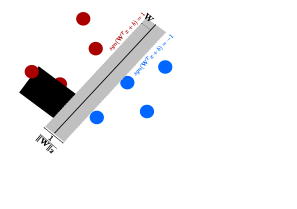
\includegraphics[scale=0.35]{IM/SVM.pdf}
  \end{center}
\end{figure}
\end{minipage}

\end{frame}
%%%%%%%%%%%%%%%%%%%%%%%%%%%%%%%%%%%%%%%%%%%%%%%%%%%%%
%%%%%%%%%%%%%%%



%%%%%%%%%%%%%%%%%%%%%%%%%%%%%%%%%%%%%%%%%%%%%%%%%%%%%
%%%%%%%%%%%%%%%%%%%%%%%%%%%%%%%%%%%%%%%%%%%%%%%%%%%%%
\begin{frame}%[Active Query]
\frametitle{Active Learning: Query Strategy}


Select the new  possible samples from the pool:
\vspace*{0.5cm}


\begin{figure}
  \begin{center}
    \includegraphics[scale=0.39]{IM/SELECTION_P.pdf}
  \end{center}
\end{figure}
\begin{minipage}{0.45\textwidth}
\centering
Unlabeled Pool
\end{minipage}
\hfill
\begin{minipage}{0.52\textwidth}
\centering
 \hspace{1.25cm}Samples
\end{minipage}
\end{frame}
%%%%%%%%%%%%%%%%%%%%%%%%%%%%%%%%%%%%%%%%%%%%%%%%%%%%%
%%%%%%%%%%%%%%%%%%%%%%%%%%%%%%%%%%%%%%%%%%%%

%%%%%%%%%%%%%%%%%%%%%%%%%%%%%%%%%%%%%%%%%%%%%%%%%%%%%
%%%%%%%%%%%%%%%%%%%%%%%%%%%%%%%%%%%%%%%%%%%%%%%%%%%%%
\begin{frame}%[Active Query]
\frametitle{Active Learning: Query Strategy}
\textbf{Uncertainty Sampling:}

\vspace*{0.2cm}
Query the instances about which the model is least certain about.

\vspace*{0.35cm}
\begin{minipage}{0.45\textwidth}
\begin{figure}
  \begin{center}
    \includegraphics[scale=0.35]{IM/UN_M.pdf}
  \end{center}
\end{figure}

\end{minipage}
\hfill
\begin{minipage}{0.5\textwidth}
Closer to  $\mathbf{W}$ $\rightarrow$ 
More Uncertain

\vspace*{0.2cm}
Measure uncertainty using entropy
\begin{equation*}
    Q(\mathbf{x}_{i}) = \sum_{j\in \mathcal{Y}}-P(y_{j}|\mathbf{x}_{i})\log\left(P(y_{j}|\mathbf{x}_{i})\right)
\end{equation*}
Probability of being in class $y_{j}$:
\begin{equation*}
    P(y_{j}|\mathbf{x}_{i})=\frac{1}{1+e^{-y_{j}W^{T}\mathbf{x}_{i}}}
\end{equation*}


\end{minipage}
\end{frame}
%%%%%%%%%%%%%%%%%%%%%%%%%%%%%%%%%%%%%%%%%%%%%%%%%%%%%
%%%%%%%%%%%%%%%%%%%%%%%%%%%%%%%%%%%%%%%%%%%%

%%%%%%%%%%%%%%%%%%%%%%%%%%%%%%%%%%%%%%%%%%%%%%%%%%%%%
%%%%%%%%%%%%%%%%%%%%%%%%%%%%%%%%%%%%%%%%%%%%%%%%%%%%%
\begin{frame}%[Active Query]
\frametitle{Active Learning: Query Strategy}
\textbf{Uncertainty Sampling:}

\vspace{0.5cm}
\begin{minipage}{0.45\textwidth}
\begin{figure}
  \begin{center}
    \includegraphics[scale=0.35]{IM/UN_M.pdf}
  \end{center}
\end{figure}
\end{minipage}
\hfill
\begin{minipage}{0.5\textwidth}

\begin{equation*}
    Q(\mathbf{x}_1)\geq Q(\mathbf{x}_2)\geq Q(\mathbf{x}_4)\geq Q(\mathbf{x}_3) 
\end{equation*}
Select the samples that maximize the entropy:
\begin{equation}
    S^{*}=\argmax_{S:|S|\leq m} \sum_{\mathbf{x}\in S} Q(\mathbf{x})
\end{equation}

\end{minipage}
\end{frame}
%%%%%%%%%%%%%%%%%%%%%%%%%%%%%%%%%%%%%%%%%%%%%%%%%%%%%
%%%%%%%%%%%%%%%%%%%%%%%%%%%%%%%%%%%%%%%%%%%%%%%%%%%%%
%%%%%%%%%


%%%%%%%%%%%%%%%%%%%%%%%%%%%%%%%%%%%%%%%%%%%%%%%%%%%%%
%%%%%%%%%%%%%%%%%%%%%%%%%%%%%%%%%%%%%%%%%%%%%%%%%%%%%
\begin{frame}%[Active Query]
\frametitle{Active Learning: Query Strategy }

\begin{center}
 \textbf{Can lead to redundant samples}   
\end{center}


\begin{figure}
  \begin{center}
  \vspace{-0.5cm}
    \includegraphics[scale=0.4]{IM/SELECTING.pdf}
  \end{center}
\end{figure}

\begin{center}
    $x_1$ is too close to  the  samples in $S_{0}$.
\end{center}


\end{frame}
%%%%%%%%%%%%%%%%%%%%%%%%%%%%%%%%%%%%%%%%%%%%%%%%%%%%%
%%%%%%%%%%%%%%%%%%%%%%%%%%%%%%%%%%%%%%%%%%%%%%%%%%%%%



%%%%%%%%%%%%%%%%%%%%%%%%%%%%%%%%%%%%%%%%%%%%%%%%%%%%%
%%%%%%%%%%%%%%%%%%%%%%%%%%%%%%%%%%%%%%%%%%%%%%%%%%%%%
\begin{frame}%[Active Query]
\frametitle{Active Learning: Query Strategy }


Other approaches:
\begin{enumerate}[\color{bar}\bfseries $\bullet$]
    \item Query-by-Committee 
    \item Expected model change
\end{enumerate}

Use graph theory to exploit the geometry of the space.

   \begin{figure}
  \begin{center}
  \vspace{0.2cm}
    \includegraphics[scale=0.4]{IM/FG.pdf}
  \end{center}
\end{figure}

\end{frame}
%%%%%%%%%%%%%%%%%%%%%%%%%%%%%%%%%%%%%%%%%%%%%%%%%%%%%
%%%%%%%%%%%%%%%%%%%%%%%%%%%%%%%%%%%%%%%%%%%%%%%%%%%%%

%%%%%%%%%%%%%%%%%%%%%%%%%%%%%%%%%%%%%%%%%%%%%%%%%%%%%
%%%%%%%%%%%%%%%%%%%%%%%%%%%%%%%%%%%%%%%%%%%%%%%%%%%%%
%\begin{frame}%[Active Query]
%\frametitle{Active Learning: Query Strategy}
%\textbf{Query-By-Committee:}

%Construct $C$ models and query the instances about which the models disagree the most 
%\vspace*{-0.2cm}
% \begin{figure}
%     \centering
%     \includegraphics[scale=0.4]{IM/COM.png}
% \end{figure}
%\end{frame}
%%%%%%%%%%%%%%%%%%%%%%%%%%%%%%%%%%%%%%%%%%%%%%%%%%%%%
%%%%%%%%%%%%%%%%%%%%%%%%%%%%%%%%%%%%%%%%%%%%%%%%%%%%%


%%%%%%%%%%%%%%%%%%%%%%%%%%%%%%%%%%%%%%%%%%%%%%%%%%%%%
%%%%%%%%%%%%%%%%%%%%%%%%%%%%%%%%%%%%%%%%%%%%%%%%%%%%%
%\begin{frame}%[Active Query]
%\frametitle{Active Learning: Query Strategy}
%\textbf{Expected Model Change:}
%Select the instance that would modify the model the most if it new its label.
%\vspace*{-0.5cm}
% \begin{figure}
%     \centering
%     \includegraphics[scale=0.36]{IM/MCM.png}
% \end{figure}
%\end{frame}
%%%%%%%%%%%%%%%%%%%%%%%%%%%%%%%%%%%%%%%%%%%%%%%%%%%%%
%%%%%%%%%%%%%%%%%%%%%%%%%%%%%%%%%%%%%%%%%%%%%%%%%%%%%



%%%%%%%%%%%%%%%%%%%%%%%%%%%%%%%%%%%%%%%%%%%%%%%%%%%%%
%%%%%%%%%%%%%%%%%%%%%%%%%%%%%%%%%%%%%%%%%%%%%%%%%%%%%
\begin{frame}%[Gaph]
\frametitle{Graph}
A Graph is a mathematical representation of objects and their relations. 
 \begin{figure}
     \centering
     \includegraphics[scale=0.5]{IM/GRAPH.pdf}
 \end{figure}

\end{frame}
%%%%%%%%%%%%%%%%%%%%%%%%%%%%%%%%%%%%%%%%%%%%%%%%%%%%%
%%%%%%%%%%%%%%%%%%%%%%%%%%%%%%%%%%%%%%%%%%%%%%%%%%%%%


%%%%%%%%%%%%%%%%%%%%%%%%%%%%%%%%%%%%%%%%%%%%%%%%%%%%%
%%%%%%%%%%%%%%%%%%%%%%%%%%%%%%%%%%%%%%%%%%%%%%%%%%%%%
\begin{frame}%[AGraph Matrix]
\frametitle{Matrix representation of a graph:}

\begin{enumerate}[\color{bar}\bfseries $\bullet$]
    \item Adjacency matrix $\mathbf{A}$
       \begin{equation*}
        \mathbf{A}_{ij}=\left\{\begin{array}{ccccc}
             1 & \mbox{if } e_{ij}=1\\
             0 & \mbox{if } otherwise
        \end{array}
        \right.
    \end{equation*}
     \item Weight matrix $\mathbf{W}$
       \begin{equation*}
        \mathbf{W}_{ij}=\left\{\begin{array}{ccccc}
             W_{ij} & \mbox{if } e_{ij}=1\\
             0 & \mbox{if } otherwise
        \end{array}
        \right.
    \end{equation*}
    \item Laplacian Matrix $\mathbf{L}$
        \begin{equation*}
        \mathbf{L}=\mathbf{D}-\mathbf{W}
    \end{equation*}
\end{enumerate}

    Where $\mathbf{D}$ is a diagonal matrix with entries $\mathbf{D}_{ii}=\sum_{j=1}^{n}W_{ij}$.
\end{frame}
%%%%%%%%%%%%%%%%%%%%%%%%%%%%%%%%%%%%%%%%%%%%%%%%%%%%%
%%%%%%%%%%%%%%%%%%%%%%%%%%%%%%%%%%%%%%%%%%%%%%%%%%%%%


%%%%%%%%%%%%%%%%%%%%%%%%%%%%%%%%%%%%%%%%%%%%%%%%%%%%%
%%%%%%%%%%%%%%%%%%%%%%%%%%%%%%%%%%%%%%%%%%%%%%%%%%%%%
\begin{frame}%[Spectrum Gaph]
\frametitle{Graph Spectrum}

\begin{minipage}{0.5\textwidth}

Let $G$ be a graph:
\begin{equation*}
    Spec(G)=\{\lambda_{1},...,\lambda_{n}\}
\end{equation*}
Where $0\leq \lambda_{1}\leq...\leq \lambda_{n}$ and $\lambda_{i}$ satisfy:
\begin{equation*}
    \mathbf{L}\mathbf{v}_{i}=\lambda_{i} \mathbfl{v}_{i}
\end{equation*}
The Graph Fourier Transform (GFT) :
\vspace*{-0.25cm}
\begin{center}
    $\mathbf{U}=[\mathbf{v}_{1},...,\mathbf{v}_{n}]$
\end{center}
Let $\mathnormal{x}$  be a signal on the graph:
\begin{center}
    $\mathnormal{x}: V\rightarrow \mathbb{R}$ 
\end{center}


    \end{minipage}
    \hfill
    \begin{minipage}{0.45\textwidth}
    \centering
    Power spectrum of  $\mathnormal{x}$ :
\begin{equation*}
   \widehat{\mathnormal{x}}  =\mathbf{U}\mathnormal{x}
\end{equation*}
 \vspace*{-0.4cm}
$\mathnormal{x}$ in the Fourier domain
 \vspace*{0.2cm}
 \begin{figure}
     \centering
     \includegraphics[scale=0.23]{IM/Sig.pdf}
 \end{figure}
 \vspace*{-0.3cm}
 $\mathnormal{x}$ in the Vertex domain
  \begin{figure}
     \centering
    \hspace*{0.25cm} 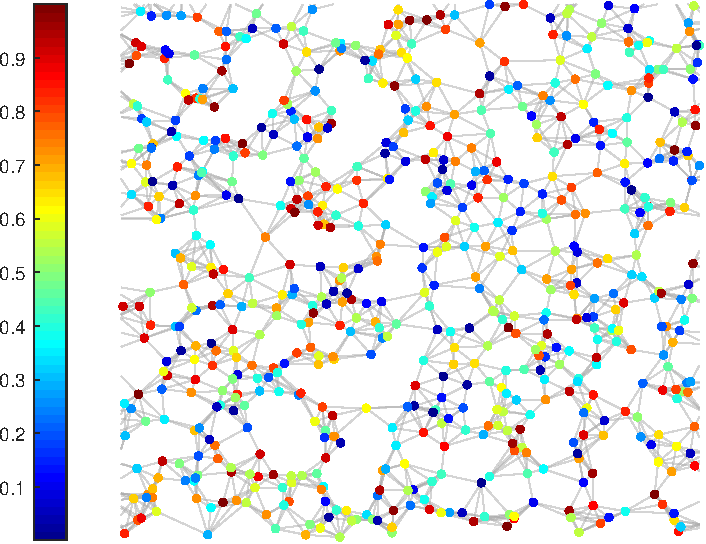
\includegraphics[scale=0.3]{IM/Sig_R.pdf}
 \end{figure}
    \end{minipage}

 
 
\end{frame}
%%%%%%%%%%%%%%%%%%%%%%%%%%%%%%%%%%%%%%%%%%%%%%%%%%%%%
%%%%%%%%%%%%%%%%%%%%%%%%%%%%%%%%%%%%%%%%%%%%%%%%%%%%%




%%%%%%%%%%%%%%%%%%%%%%%%%%%%%%%%%%%%%%%%%%%%%%%%%%%%%
%%%%%%%%%%%%%%%%%%%%%%%%%%%%%%%%%%%%%%%%%%%%%%%%%%%%%
\begin{frame}%[Sampling Gaph]
\frametitle{Sampling on Graph}

Select $m$ out of $n$ total vertices:


\vspace*{15px}
\begin{minipage}{0.5\textwidth}
\centering
Samples on the Graph
\begin{figure}
    \centering
 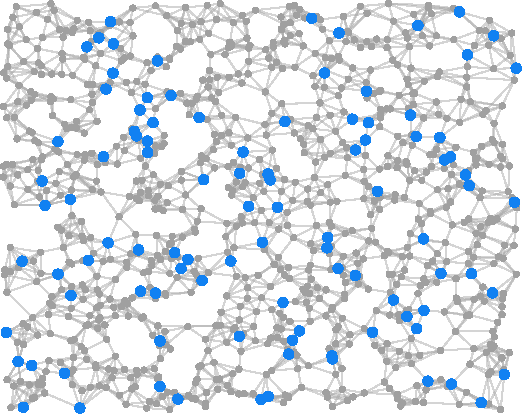
\includegraphics[scale=0.5]{IM/Samplig.pdf}
\end{figure}
    \end{minipage}
    \hfill
    \begin{minipage}{0.45\textwidth}
    \vspace*{0.5cm}
    \centering
       Pattern Spectrum
  \begin{figure}
     \centering
     \includegraphics[scale=0.37]{IM/Samplig_RAND.pdf}
 \end{figure}
    \end{minipage}

 
 
\end{frame}
%%%%%%%%%%%%%%%%%%%%%%%%%%%%%%%%%%%%%%%%%%%%%%%%%%%%%
%%%%%%%%%%%%%%%%%%%%%%%%%%%%%%%%%%%%%%%%%%%%%%%%%%%%%


%%%%%%%%%%%%%%%%%%%%%%%%%%%%%%%%%%%%%%%%%%%%%%%%%%%%%
%%%%%%%%%%%%%%%%%%%%%%%%%%%%%%%%%%%%%%%%%%%%%%%%%%%%%

\begin{frame}%[BN Sampling Gaph]
\frametitle{Blue Noise Sampling on Graph}


Select $m$ out of $n$ total vertices such that:

\begin{enumerate}[\color{bar}\bfseries 1.]
    \item The selected  nodes are equally spaced apart
    \item  Selected nodes are as far as possible from each other
\end{enumerate}

\begin{minipage}{0.5\textwidth}
\centering
Samples on the Graph
\begin{figure}
    \centering
 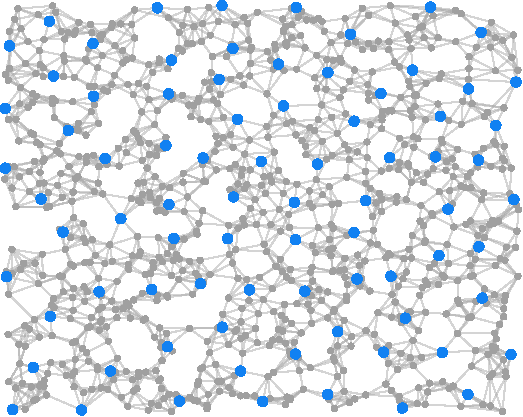
\includegraphics[scale=0.5]{IM/Samplig_RAND_BN.pdf}
\end{figure}
    \end{minipage}
    \hfill
    \begin{minipage}{0.45\textwidth}
    \vspace*{0.5cm}
    \centering
   Pattern Spectrum
  \begin{figure}
     \centering
     \includegraphics[scale=0.37]{IM/Samplig_SPC_BN.pdf}
 \end{figure}
    \end{minipage}
\centering
 Blue Noise Patterns have high-frequency power dominance.
 
\end{frame}
%%%%%%%%%%%%%%%%%%%%%%%%%%%%%%%%%%%%%%%%%%%%%%%%%%%%%
%%%%%%%%%%%%%%%%%%%%%%%%%%%%%%%%%%%%%%%%%%%%%%%%%%%%%


\begin{frame}%[BN Sampling Gaph]
\frametitle{Blue Noise Sampling on Graph}
The minimum distance between 2 vertices $\textcolor{bar}{\mathbf{    \longrightarrow}}$ shortest path $\Gamma$.

Blue Noise: 

Minimum $\Gamma$ between  selected vertices $\textcolor{bar}{\mathbf{\rightarrow}}$ principal path-length $\lambda_{b}$:


\begin{minipage}{0.5\textwidth}

\begin{equation*}
    d=\frac{1}{\mathbb{E}\{\mathcal{N}(\lambda_{b})\}}
\end{equation*}

Where $\mathbb{E}\{\mathcal{N}(\lambda_{b})\}$ is the expected number of nodes at a path length $\lambda_{b}$ of a selected node.

\begin{center}
    $\mathbb{E}\{\mathcal{N}(\lambda_{b})\}\rightarrow$ Graph dependent
\end{center}

    \end{minipage}
    \hfill
    \begin{minipage}{0.45\textwidth}
    \vspace*{0.5cm}
    \centering

  \begin{figure}
     \centering
     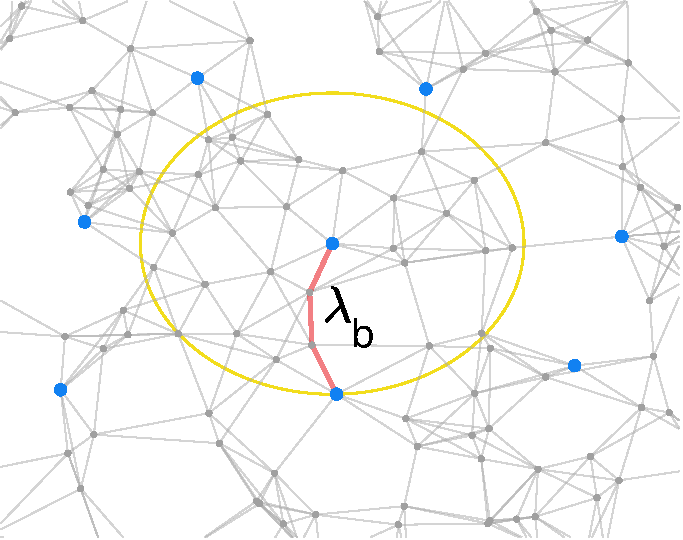
\includegraphics[scale=0.37]{IM/PATH.pdf}
 \end{figure}
    \end{minipage}


\end{frame}
%%%%%%%%%%%%%%%%%%%%%%%%%%%%%%%%%%%%%%%%%%%%%%%%%%%%%
%%%%%%%%%%%%%%%%%%%%%%%%%%%%%%%%%%%%%%%%%%%%%%%%%%%%%

%%%%%%%%%%%%%%%%%%%%%%%%%%%%%%%%%%%%%%%%%%%%%%%%%%%%%
%%%%%%%%%%%%%%%%%%%%%%%%%%%%%%%%%%%%%%%%%%%%%%%%%%%%%
\begin{frame}%[Problem]
\frametitle{Active Learning: Problem Formulation}

Given an original set of labeled points $S^{0}$ select  $m$ points in $S^{1}$  such that the future expected  loss is minimized:
\begin{equation}
    \min_{S^{1}:|S|\leq m} \mathbb{E}_{\mathbf{x},y~\mathnormal{p}_{z}}[\ell(\mathbf{x},y;A_{S^0 \cup S^{1}})]
\end{equation}
Where $x$ are all the data points and $y$ its respective class $\ell$ is the lost function, $A$ is the learned algorithm.


\end{frame}
%%%%%%%%%%%%%%%%%%%%%%%%%%%%%%%%%%%%%%%%%%%%%%%%%%%%%
%%%%%%%%%%%%%%%%%%%%%%%%%%%%%%%%%%%%%%%%%%%%%%%%%%%%%


%%%%%%%%%%%%%%%%%%%%%%%%%%%%%%%%%%%%%%%%%%%%%%%%%%%%%
%%%%%%%%%%%%%%%%%%%%%%%%%%%%%%%%%%%%%%%%%%%%%%%%%%%%%
\begin{frame}%[Problem]
\frametitle{Active Learning: Problem Formulation}

In Passive Learning, the future expected  loss can be bounded by:
\begin{multline*}
    \mathbb{E}_{\mathbf{x},y~\mathnormal{p}_{z}}[\ell(\mathbf{x},y;A_{S})]\leq \underbrace{\left|\mathbb{E}_{\mathbf{x},y~\mathnormal{p}_{z}}[\ell(\mathbf{x},y;A_{S})]\right|}_{\text{Generalization Error}}+\underbrace{\left|\frac{1}{|S|}\sum_{j\in S}\ell(\mathbf{x}_{j},y_{j};A_{S})\right|}_{\text{Training Error}}
\end{multline*}
\begin{figure}
    \centering
    \includegraphics[scale=0.4]{IM/VAR_BIAS_CORE_P.pdf}
\end{figure}

\end{frame}
%%%%%%%%%%%%%%%%%%%%%%%%%%%%%%%%%%%%%%%%%%%%%%%%%%%%%
%%%%%%%%%%%%%%%%%%%%%%%%%%%%%%%%%%%%%

%%%%%%%%%%%%%%%%%%%%%%%%%%%%%%%%%%%%%%%%%%%%%%%%%%%%%
%%%%%%%%%%%%%%%%%%%%%%%%%%%%%%%%%%%%%%%%%%%%%%%%%%%%%
\begin{frame}%[Problem]
\frametitle{Active Learning: Problem Formulation}


In Active Learning, the future expected  loss can be bounded by:
\begin{multline*}
    \mathbb{E}_{\mathbf{x},y~\mathnormal{p}_{z}}[\ell(\mathbf{x},y;A_{S})]\leq \underbrace{\left|\mathbb{E}_{\mathbf{x},y~\mathnormal{p}_{z}}[\ell(\mathbf{x},y;A_{S})]-\textcolor{Blue}{\frac{1}{n}\sum_{i\in [n]}\ell(\mathbf{x}_{i},y_{i};A_{S})}\right|}_{\text{Generalization Error}}+...\\
    ...+\underbrace{\left|\frac{1}{|S|}\sum_{j\in S}\ell(\mathbf{x}_{j},y_{j};A_{S})\right|}_{\text{Training Error}}+\underbrace{\textcolor{Blue}{\left|\frac{1}{n}\sum_{i\in [n]}\ell(\mathbf{x}_{i},y_{i};A_{S})-\frac{1}{|S|}\sum_{j\in S}\ell(\mathbf{x}_{j},y_{j};A_{S})\right|}}_{\text{Core Error}}
\end{multline*}

Where $n$ is total number of points in the unlabeled pool
\end{frame}
%%%%%%%%%%%%%%%%%%%%%%%%%%%%%%%%%%%%%%%%%%%%%%%%%%%%%
%%%%%%%%%%%%%%%%%%%%%%%%%%%%%%%%%%%%%%%%%%%%%%%%%%%%%


%%%%%%%%%%%%%%%%%%%%%%%%%%%%%%%%%%%%%%%%%%%%%%%%%%%%%
%%%%%%%%%%%%%%%%%%%%%%%%%%%%%%%%%%%%%%%%%%%%%%%%%%%%%
\begin{frame}%[Problem]
\frametitle{Active Learning: Problem Formulation}

\begin{figure}
    \centering
    \includegraphics[scale=0.4]{IM/VAR_BIAS_CORE.pdf}
\end{figure}
\end{frame}
%%%%%%%%%%%%%%%%%%%%%%%%%%%%%%%%%%%%%%%%%%%%%%%%%%%%%
%%%%%%%%%%%%%%%%%%%%%%%%%%%%%%%%%%%%%%%%%%%%%%%%%%%%%

%%%%%%%%%%%%%%%%%%%%%%%%%%%%%%%%%%%%%%%%%%%%%%%%%%%%%
%%%%%%%%%%%%%%%%%%%%%%%%%%%%%%%%%%%%%%%%%%%%%%%%%%%%%
\begin{frame}%[Problem]
\frametitle{Active Learning: Problem Formulation}
Note that:
\begin{enumerate}[\color{bar}\bfseries 1.]
    \item Generalization Error ($E$): bounded for several Machine Learning Algorithms
    \item Training error: $E_{in}= 0$
\end{enumerate}
Then focus in core error $E_{core}$: 
\begin{figure}
    \centering
    \includegraphics[scale=0.48]{IM/eq.pdf}
\end{figure}
\begin{center}
    \textcolor{UdelRed}{\textbf{We don't know $\mathnormal{y_{i}}$}}
\end{center}
\end{frame}
%%%%%%%%%%%%%%%%%%%%%%%%%%%%%%%%%%%%%%%%%%%%%%%%%%%%%
%%%%%%%%%%%%%%%%%%%%


%%%%%%%%%%%%%%%%%%%%%%%%%%%%%%%%%%%%%%%%%%%%%%%%%%%%%
%%%%%%%%%%%%%%%%%%%%%%%%%%%%%%%%%%%%%%%%%%%%%%%%%%%%%
\begin{frame}%[BOUND Core error]
\frametitle{Core Error Bound}
 $E_{in}=0$ then:
\begin{equation*}
   E_{core} = \frac{1}{n}\sum_{i\in [n]}\ell(\mathbf{x}_{i},y_{i};A_{S})
\end{equation*}
$\ell\rightarrow\lambda^{\mathnormal{l}}$-Lipschitz continuous and $\delta_{S}$  is a cover of the n points. With probability at least $1-\gamma$, 
\begin{equation}
    E_{core}\leq \delta (\lambda^{l}+\lambda^{\mu}LC)+\underbrace{\sqrt{\frac{L^{2}\log{1/\gamma}}{2n}}}_{Hoeffding's\;Bound}
\end{equation}
Where $\delta$ is the cover radius, $\lambda^{l}$ and $\lambda^{\mu}$ are  class distributions constants, $L$ is the Lipschitz constant and $C$ number of classes.

$f(x)$ is \textbf{$\lambda^{\mathnormal{l}}$-Lipschitz Continuous} if:
\begin{equation*}
    |f(x_{1})-f(x_{2})|\leq L
    |x_{1}-x_{2}| \;\; \foall x_{1},x_{2}\in \mathbb{R}
\end{equation*}

\end{frame}
%%%%%%%%%%%%%%%%%%%%%%%%%%%%%%%%%%%%%%%%%%%%%%%%%%%%%
%%%%%%%%%%%%%%%%%%%%



%%%%%%%%%%%%%%%%%%%%%%%%%%%%%%%%%%%%%%%%%%%%%%%%%%%%%
%%%%%%%%%%%%%%%%%%%%%%%%%%%%%%%%%%%%%%%%%%%%%%%%%%%%%
\begin{frame}%[BOUND Core error]
\frametitle{Core Error Bound}
\begin{center}
  $    \delta \longrightarrow$ Point  location  
\end{center}

Sparsity between the points in $S$ minimize $\delta$.
\begin{figure}
    \centering
    \includegraphics[scale=0.35]{IM/DELTA.pdf}
\end{figure}
\end{frame}
%%%%%%%%%%%%%%%%%%%%%%%%%%%%%%%%%%%%%%%%%%%%%%%%%%%%%
%%%%%%%%%%%%%%%%%%%%

%%%%%%%%%%%%%%%%%%%%%%%%%%%%%%%%%%%%%%%%%%%%%%%%%%%%%
%%%%%%%%%%%%%%%%%%%%%%%%%%%%%%%%%%%%%%%%%%%%%%%%%%%%%
\begin{frame}%[BOUND Core error]
\frametitle{Optimization problem:}

 Using the upper bound the problem active learning problem becomes:
 
 \begin{equation}
     \min_{S^{1}:|S^{1}|\leq m} \delta(S^{0}\cup S^{1})
 \end{equation}
\begin{enumerate}[\color{bar}\bfseries $\bullet$]
    \item Equivalent to the min-max facility location problem
    \item NP hard
    \item Maximize the distance between points in $S^{0}\cup S^{1}$
\end{enumerate}
 
\end{frame}
%%%%%%%%%%%%%%%%%%%%%%%%%%%%%%%%%%%%%%%%%%%%%%%%%%%%%
%%%%%%%%%%%%%%%%%%%%


%%%%%%%%%%%%%%%%%%%%%%%%%%%%%%%%%%%%%%%%%%%%%%%%%%%%%
%%%%%%%%%%%%%%%%%%%%%%%%%%%%%%%%%%%%%%%%%%%%%%%%%%%%%
\begin{frame}%[BOUND Core error]
\frametitle{Optimization problem:}
Maximize the distance between points in $S^{0}\cup S^{1}$:
\begin{figure}
    \centering
    \includegraphics[scale=0.4]{IM/SEPARATION.pdf}

\end{figure}
\centering
$\delta_{S2}<\delta_{S1}$
\end{frame}
%%%%%%%%%%%%%%%%%%%%%%%%%%%%%%%%%%%%%%%%%%%%%%%%%%%%%
%%%%%%%%%%%%%%%%%%%%


%%%%%%%%%%%%%%%%%%%%%%%%%%%%%%%%%%%%%%%%%%%%%%%%%%%%%
%%%%%%%%%%%%%%%%%%%%%%%%%%%%%%%%%%%%%%%%%%%%%%%%%%%%%
\begin{frame}%[BN COVER]
\frametitle{Blue Noise on Graph and the Optimization problem:}
Definition of Blue Noise on graph:
\begin{definition}
$S$ is Blue Noise pattern if:

\begin{enumerate}
    \item[$\bullet$] There is a collection collection of  balls $B(s_{i},\delta)$ that forms a cover of $V(G)$
    \item[$\bullet$]  $\delta$ is  minimum 
\end{enumerate}
\end{definition}

\begin{huge}
\begin{equation*}
    \delta \sim \lambda_{b}
\end{equation*}
\end{huge}

\end{frame}
%%%%%%%%%%%%%%%%%%%%%%%%%%%%%%%%%%%%%%%%%%%%%%%%%%%%%
%%%%%%%%%%%%%%%%%%%%%%%%%%%%%%%%%%%%%%%%%%%%%%%%%%%%%

%%%%%%%%%%%%%%%%%%%%%%%%%%%%%%%%%%%%%%%%%%%%%%%%%%%%%
%%%%%%%%%%%%%%%%%%%%%%%%%%%%%%%%%%%%%%%%%%%%%%%%%%%%%


%%%%%%%%%%%%%%%%%%%%%%%%%%%%%%%%%%%%%%%%%%%%%%%%%%%%%
%%%%%%%%%%%%%%%%%%%%%%%%%%%%%%%%%%%%%%%%%%%%%%%%%%%%%
\begin{frame}%[VAC]

\frametitle{Blue Noise and Active learning}
\textbf{Step 1}

 Initialize $S^{0}$ with blue noise using Void and Cluster:

\begin{figure}
    \centering
    \includegraphics[scale=0.35]{IM/VA.pdf}
   
\end{figure}



\end{frame}

%%%%%%%%%%%%%%%%%%%%%%%%%%%%%%%%%%%%%%%%%%%%%%%%%%%%%
%%%%%%%%%%%%%%%%%%%%%%%%%%%%%%%%%%%%%%%%%%%%%%%%%%%%%
%%%%%%%%%%%%%%%%%%%

%%%%%%%%%%%%%%%%%%%%%%%%%%%%%%%%%%%%%%%%%%%%%%%%%%%%%
%%%%%%%%%%%%%%%%%%%%%%%%%%%%%%%%%%%%%%%%%%%%%%%%%%%%%
\begin{frame}%[BOUND Core error]
\frametitle{Blue Noise and Active learning}
\textbf{Step 2:}

\vspace{0.2cm}
     Select the $m$ points with the largest uncertainty such that the shortest path between all selected points is greater than $\lambda_{b}$:

\vspace{0.25cm}
\begin{minipage}{0.55\textwidth}
\vspace{-0.7cm}
\begin{small}
    \begin{maxi*}|l|
  {S^{1}:|S^{1}|\leq m}{\sum_{j\in S}\sum_{i \in \mathcal{Y}}Q(\mathbf{x}_j,y_i)}{}{}
  \addConstraint{\Gamma_{ij}\geq \lambda_{b} \;\; \forall i,j \in S^{0}\cup S^{1}} 
\end{maxi*}
Where :
\begin{equation*}
    Q(x_j,y_i)=-P_{\theta}(y_{i}|\mathbf{x}_{j})\log(P_{\theta}(y_{i}|\mathbf{x}_{j}))
\end{equation*}
\end{small}
    \end{minipage}
    \hfill
    \begin{minipage}{0.4\textwidth}
    \centering
\begin{figure}
    \centering
    \includegraphics[scale=0.3]{IM/model.pdf}
\end{figure}
    \end{minipage}
\end{frame}
%%%%%%%%%%%%%%%%%%%%%%%%%%%%%%%%%%%%%%%%%%%%%%%%%%%%%
%%%%%%%%%%%%%%%%%%%%%%%%%%%%%%%%%%%%%%%%%%%%%%%%%%%%%


%%%%%%%%%%%%%%%%%%%%%%%%%%%%%%%%%%%%%%%%%%%%%%%%%%%%%
%%%%%%%%%%%%%%%%%%%%%%%%%%%%%%%%%%%%%%%%%%%%%%%%%%%%%
\begin{frame}%[SR]
\frametitle{Signal Reconstruction as a Classifier}
\begin{minipage}{0.45\textwidth}
\centering
Class Function

Band-width=$n$
\vspace{0.3cm}
\begin{figure}
    \centering
 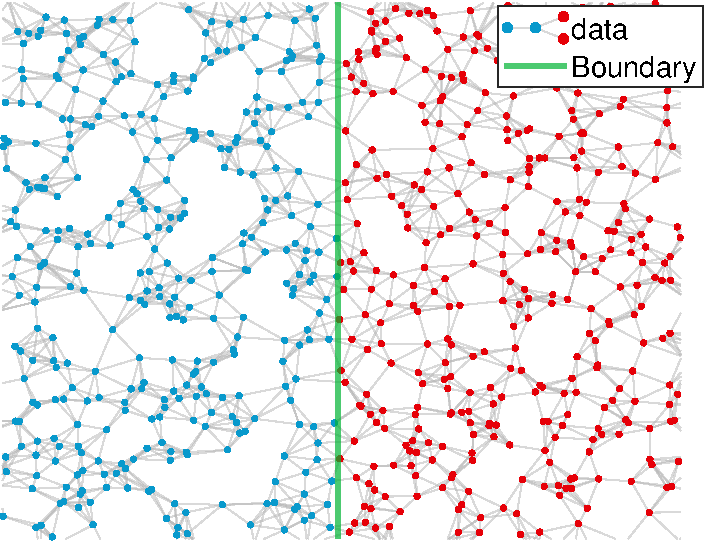
\includegraphics[scale=0.4]{IM/CLAS.pdf}
\end{figure}
    \end{minipage}
    \hfill
    \begin{minipage}{0.45\textwidth}
    \centering
    Smooth Signal
    
Band-width=$0.05n$
  \begin{figure}
     \centering
     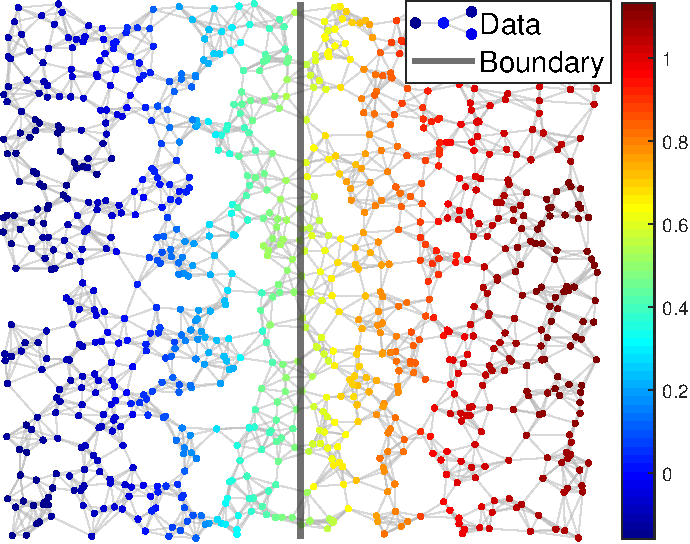
\includegraphics[scale=0.4]{IM/SMOOTH.pdf}
 \end{figure}
    \end{minipage}
\begin{center}
    Class Function $\approx$ Smooth Signal
\end{center}

\end{frame}

%%%%%%%%%%%%%%%%%%%%%%%%%%%%%%%%%%%%%%%%%%%%%%%%%%%%%
%%%%%%%%%%%%%%%%%%%%%%%%%%%%%%%%%%%%%%%%%%%%%%%%%%%%%

%%%%%%%%%%%%%%%%%%%%%%%%%%%%%%%%%%%%%%%%%%%%%%%%%%%%%
%%%%%%%%%%%%%%%%%%%%%%%%%%%%%%%%%%%%%%%%%%%%%%%%%%%%%
\begin{frame}%[SR]
\frametitle{Signal Reconstruction as a Classifier}

A signal $\mathnormal{x}$ can be reconstructed using the values of $\mathnormal{x}$ in $S$ ($S \subset V)$ if:

\begin{equation*}
    \mathnormal{x}_{rec}=\argmin_{z\in span(\mathbf{U}_{k})}\parallel \mathbf{M}z-\mathnormal{x}(S)\parallel_{2}^{2}
\end{equation*}

\begin{equation*}
    \mathnormal{x}_{rec}=\mathbf{U}_{k}(\mathbf{MU}_{k})^{\dagger}\mathnormal{x}
\end{equation*}

Where $\mathbf{U}_{k}$ contain the first $k$ eigenvectors, $\mathbf{M}=[\delta_{s_1},\delta_{s_2},...,\delta_{s_m}]^{T}$ and $delta_{v}$ is the $n$ dimensional Kronecker column vector centered at $v$ .


Classify an instance using a threshold function  in $\mathnormal{x}_{rec}$.
\end{frame}


%%%%%%%%%%%%%%%%%%%%%%%%%%%%%%%%%%%%%%%%%%%%%%%%%%%%%
%%%%%%%%%%%%%%%%%%%%%%%%%%%%%%%%%%





%%%%%%%%%%%%%%%%%%%%%%%%%%%%%%%%%%%%%%%%%%%%%%%%%%%%%
%%%%%%%%%%%%%%%%%%%%%%%%%%%%%%%%%%%%%%%%%%%%%%%%%%%%%
\begin{frame}%[VAC]
\frametitle{Experiments: Data}
Four synthetic data experiments with 2 classes:
\begin{enumerate} [\color{bar}\bfseries 1.]
    \item Linearly separable data in 2-D
    \item Non-linearly separable data in 2-D
    \item Non-linearly separable data in 3-D
    \item Non-Separable data in 2-D
\end{enumerate}

Build the graph connecting each observation to its 6 nearest neighbors.
\end{frame}

%%%%%%%%%%%%%%%%%%%%%%%%%%%%%%%%%%%%%%%%%%%%%%%%%%%%%
%%%%%%%%%%%%%%%%%%%%%%%%%%%%%%%%%%%%%%%%%%%%%%%%%%%%%



%%%%%%%%%%%%%%%%%%%%%%%%%%%%%%%%%%%%%%%%%%%%%%%%%%%%%
%%%%%%%%%%%%%%%%%%%%%%%%%%%%%%%%%%%%%%%%%%%%%%%%%%%%%
\begin{frame}%[VAC]
\frametitle{Experiments: Algorithms }
Methods of evaluation:

\begin{enumerate} [\color{bar}\bfseries 1.]
    \item Passive SVM (Random Sampling) 
    \item Passive Signal Reconstruction (Random Sampling) 
    \item Active Learning: Uncertainty Sampling SVM
    \item Active Learning: Uncertainty and Blue Noise Sampling SVM
     \item Active Learning: Uncertainty and Blue Noise Sampling Signal Reconstruction
\end{enumerate}

For signal Reconstruction, we assume the band-with of the signal contains $5\%$ of the spectrum. 
\end{frame}

%%%%%%%%%%%%%%%%%%%%%%%%%%%%%%%%%%%%%%%%%%%%%%%%%%%%%
%%%%%%%%%%%%%%%%%%%%%%%%%%%%%%%%%%%%%%%%%%%%%%%%%%%%%


%%%%%%%%%%%%%%%%%%%%%%%%%%%%%%%%%%%%%%%%%%%%%%%%%%%%%
%%%%%%%%%%%%%%%%%%%%%%%%%%%%%%%%%%%%%%%%%%%%%%%%%%%%%
\begin{frame}%[VAC]
\frametitle{Data}

\begin{figure}[ht]
 \begin{tabular}{cc}
   \includegraphics[scale=0.4]{DATA/DATAS.pdf} &
    \includegraphics[scale=0.4]{DATA/CLASS_NLS.pdf}
   \\
    (a) Linearly Separable 2D & (b) Non-linearly separable 2D\\
 \end{tabular}
 \bigskip
 \caption{Data Sets}
\end{figure}
\end{frame}

%%%%%%%%%%%%%%%%%%%%%%%%%%%%%%%%%%%%%%%%%%%%%%%%%%%%%
%%%%%%%%%%%%%%%%%%%%%%%%%%%%%%%%%%%%%%%%%%%%%%%%%%%%%

\begin{frame}%[VAC]
\frametitle{Accuracy}

\begin{figure}[ht]
 \begin{tabular}{cc}
   \includegraphics[scale=0.4]{ACC/ERROR_INA.pdf} &
    \includegraphics[scale=0.4]{ACC/ACUR_NS2.pdf}
   \\
    (a) Linearly Separable 2D & (b) Non-linearly separable 2D\\
 \end{tabular}
 \bigskip
 
\end{figure}
\end{frame}
%%%%%%%%%%%%%%%%%%%%%%%%%%%%%%%%%%%%%%%%%%%%%%%%%%%%%

%%%%%%%%%%%%%%%%%%%%%%%%%%%%%%%%%%%%%%%%%%%%%%%%%%%%%
%%%%%%%%%%%%%%%%%%%%%%%%%%%%%%%%%%%%%%%%%%%%%%%%%%%%%

\begin{frame}%[VAC]
\frametitle{SVM: Blue Noise Vs Uncertainty}
\begin{figure}[ht]
 \begin{tabular}{cc}
   \includegraphics[scale=0.425]{BN_VS_UN/UN.png} &
    \includegraphics[scale=0.35]{BN_VS_UN/SVM_BN.png}
   \\
    (a) Uncertainty Sampling & (b) Blue Noise\\
 \end{tabular}
 \bigskip
 \caption{Blue Noise Vs Uncertainty in SVM}
\end{figure}
\end{frame}
%%%%%%%%%%%%%%%%%%%%%%%%%%%%%%%%%%%%%%%%%%%%%%%%%%%%%



%%%%%%%%%%%%%%%%%%%%%%%%%%%%%%%%%%%%%%%%%%%%%%%%%%%%%
%%%%%%%%%%%%%%%%%%%%%%%%%%%%%%%%%%%%%%%%%%%%%%%%%%%%%

\begin{frame}%[VAC]
\frametitle{Boundary Detection and $\delta$ redunction}
\begin{figure}[ht]
 \begin{tabular}{cc}
   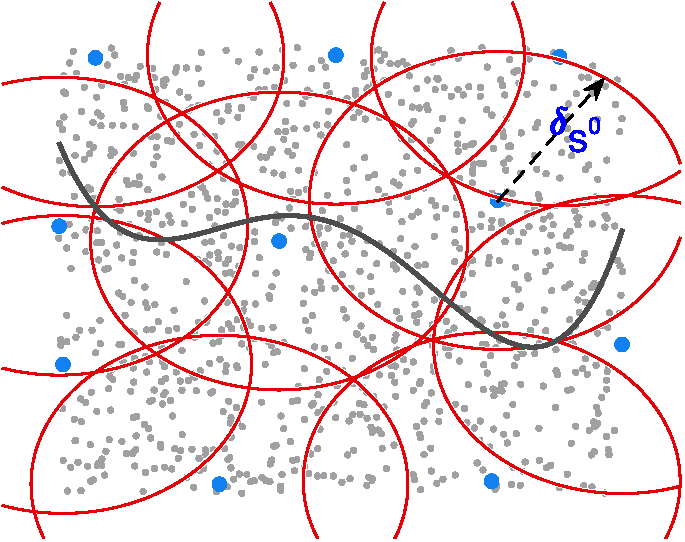
\includegraphics[scale=0.4]{BOUND/COVER.pdf} &
    \includegraphics[scale=0.4]{BOUND/SELECTION_PROCES.pdf}
   \\
    (a) Cover (ratio=0.01) & (b) Bound detection (ratio=0.047)\\
 \end{tabular}
 \bigskip
\end{figure}
\end{frame}
%%%%%%%%%%%%%%%%%%%%%%%%%%%%%%%%%%%%%%%%%%%%%%%%%%%%%


%%%%%%%%%%%%%%%%%%%%%%%%%%%%%%%%%%%%%%%%%%%%%%%%%%%%%
%%%%%%%%%%%%%%%%%%%%%%%%%%%%%%%%%%%%%%%%%%%%%%%%%%%%%
\begin{frame}%[VAC]
\frametitle{Data}

\begin{figure}[ht]
 \begin{tabular}{cc}
     \includegraphics[scale=0.4]{DATA/DATA_3D.pdf} &
    \includegraphics[scale=0.4]{DATA/CLASSNS.pdf}
   \\
    (a) Non-linearly separable 3D& (b)Non-Separable 2D \\
 \end{tabular}
 \bigskip
 \caption{Data Sets}
\end{figure}
\end{frame}

%%%%%%%%%%%%%%%%%%%%%%%%%%%%%%%%%%%%%%%%%%%%%%%%%%%%%
%%%%%%%%%%%%%%%%%%%%%%%%%%%%%%%%%%%%%%%%%%%%%%%%%%%%%

\begin{frame}%[VAC]
\frametitle{Accuracy}

\begin{figure}[ht]
 \begin{tabular}{cc}
     \includegraphics[scale=0.4]{ACC/ACC3d.pdf} &
    \includegraphics[scale=0.4]{ACC/ERROR_NS.pdf}
   \\
    (a) Non-linearly separable 3D& (b)Non-Separable 2D \\
 \end{tabular}
 \bigskip
 
\end{figure}
\end{frame}
%%%%%%%%%%%%%%%%%%%%%%%%%%%%%%%%%%%%%%%%%%%%%%%%%%%%%



%%%%%%%%%%%%%%%%%%%%%%%%%%%%%%%%%%%%%%%%%%%%%%%%%%%%%
\begin{frame}%[VAC]
\frametitle{Conclusion a Future Work }

\begin{enumerate} [\color{bar}\bfseries 1.]
    \item Sparsity in the point selection process has mathematical support
    \item Blue-Noise Sampling minimize the $\delta_{S}$
    \item Uncertainty  helps in the boundary detection
    \item Blue noise sampling outperforms random and uncertainty sampling
    \item Compare with more recent and effective sampling techniques
    \item Implementation in real data sets
F\end{enumerate}
\end{frame}

%%%%%%%%%%%%%%%%%%%%%%%%%%%%%%%%%%%%%%%%%%%%%%%%%%%%%
%%%%%%%%%%%%%%%%%%%%%%%%%%%%%%%%%%%%%%%%%%%%%%%%%%%%%


\begin{frame}
\frametitle{Bibliography}

\begin{small}
    
\begin{thebibliography}{10}
\bibitem{Nowak}
\alert{Castro, Rui M and Nowak, Robert D}
\newblock {Minimax bounds for active learning}
\newblock {\em IEEE Transactions on Information Theory, 54(5), 2339--2353, 2008}.
\bibitem{Active}
\alert{Settles, Burr}
\newblock  {Active learning literature survey}
\newblock {\em SUniversity of Wisconsin-Madison Department of Computer Sciences, 2009}.
\bibitem{blue}
\alert{Parada-Mayorga, Alejandro and Lau, Daniel L and Giraldo, Jhony H and Arce, Gonzalo R}
\newblock {Blue-Noise Sampling on Graphs}
\newblock {\em IEEE Transactions on Signal and Information Processing over Networks, 5(2): 554--569, 2019}.
\bibitem{Core}
\alert{Sener, Ozan and Savarese, Silvio}
\newblock {Active learning for convolutional neural networks: A core-set approach}
\newblock {\em arXiv preprint arXiv:1708.00489,2017}.

\end{thebibliography}

\end{small}

\end{frame}

\end{document} 
